\chapter{Figures}
\label{sec:Appendix}

\begin{figure}
	\begin{center}
		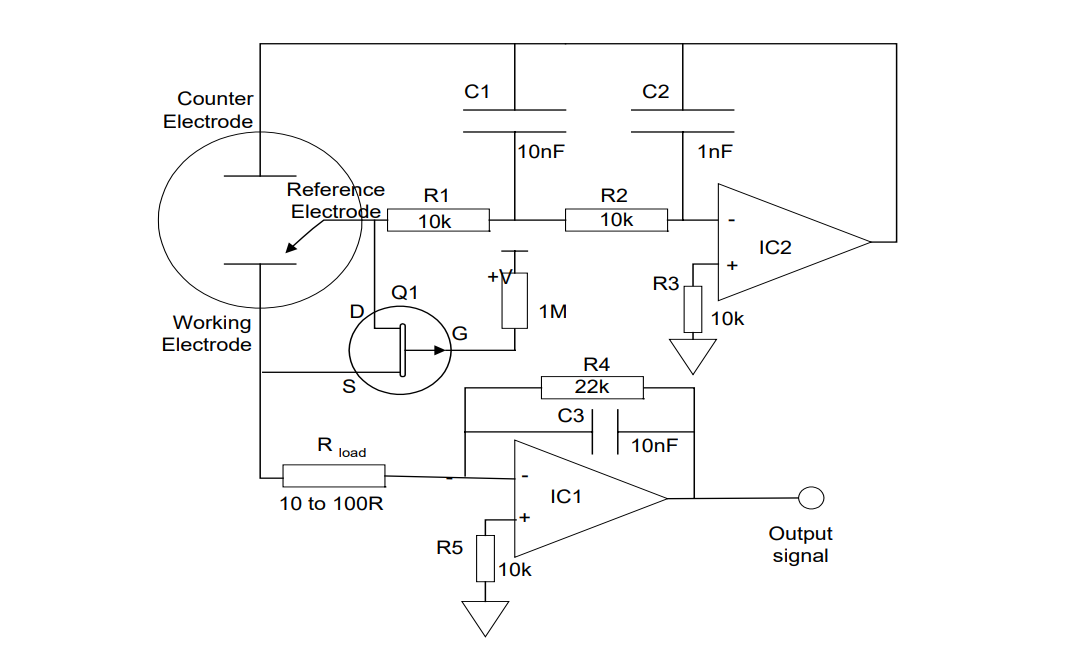
\includegraphics[width=1\textwidth]{Pics/8}
		\caption{Initial Circuit Schematic}
		\label{fig:A.1}
		\vspace{1.2cm}
		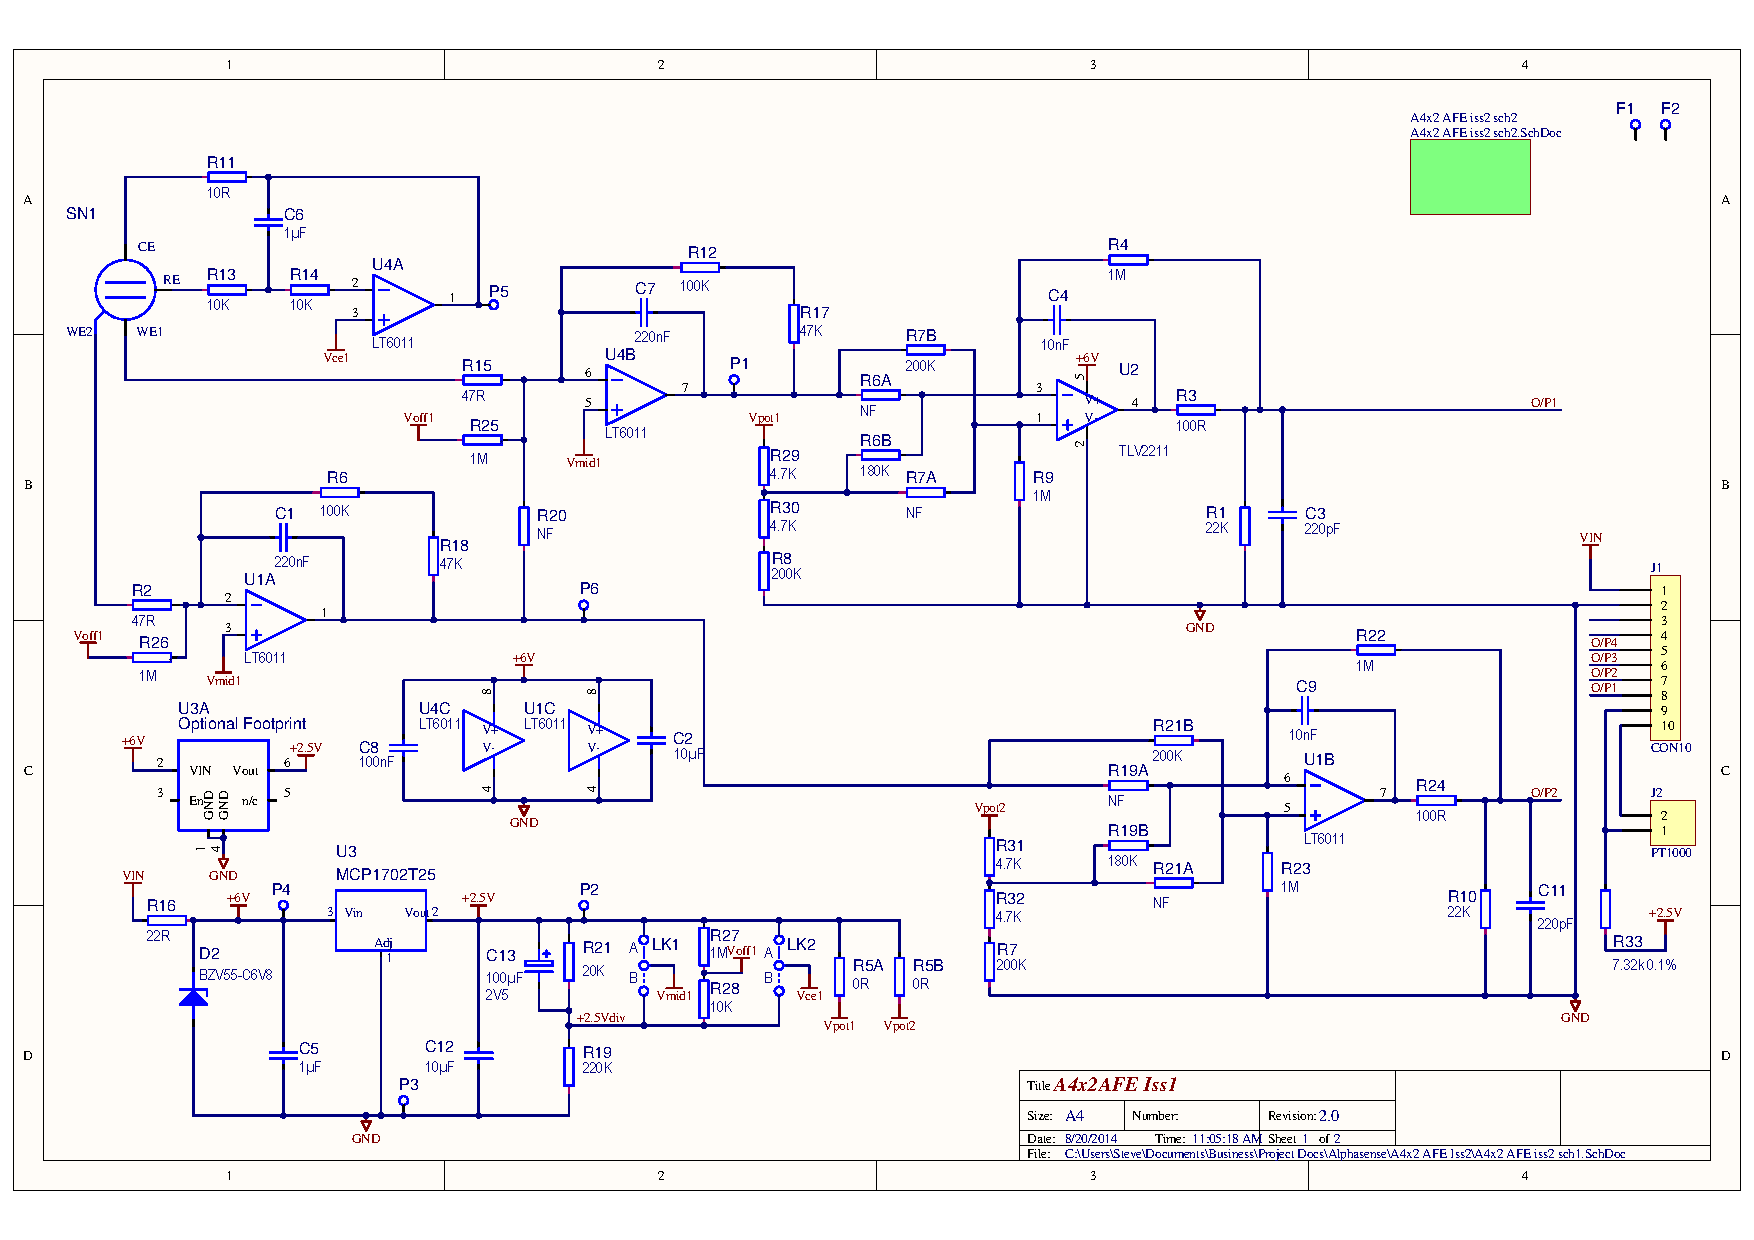
\includegraphics[page=1,width=1\textwidth]{Pics/5.pdf}
		\label{fig:A.2}
		\caption{ISB Board Circuit Schematic}
		%\small
		%Explanation
	\end{center}
\end{figure}



	
%	\begin{figure}[h]
%		\centering
%		\begin{tabular}{@{}c@{\hspace{.5cm}}c@{}}
%			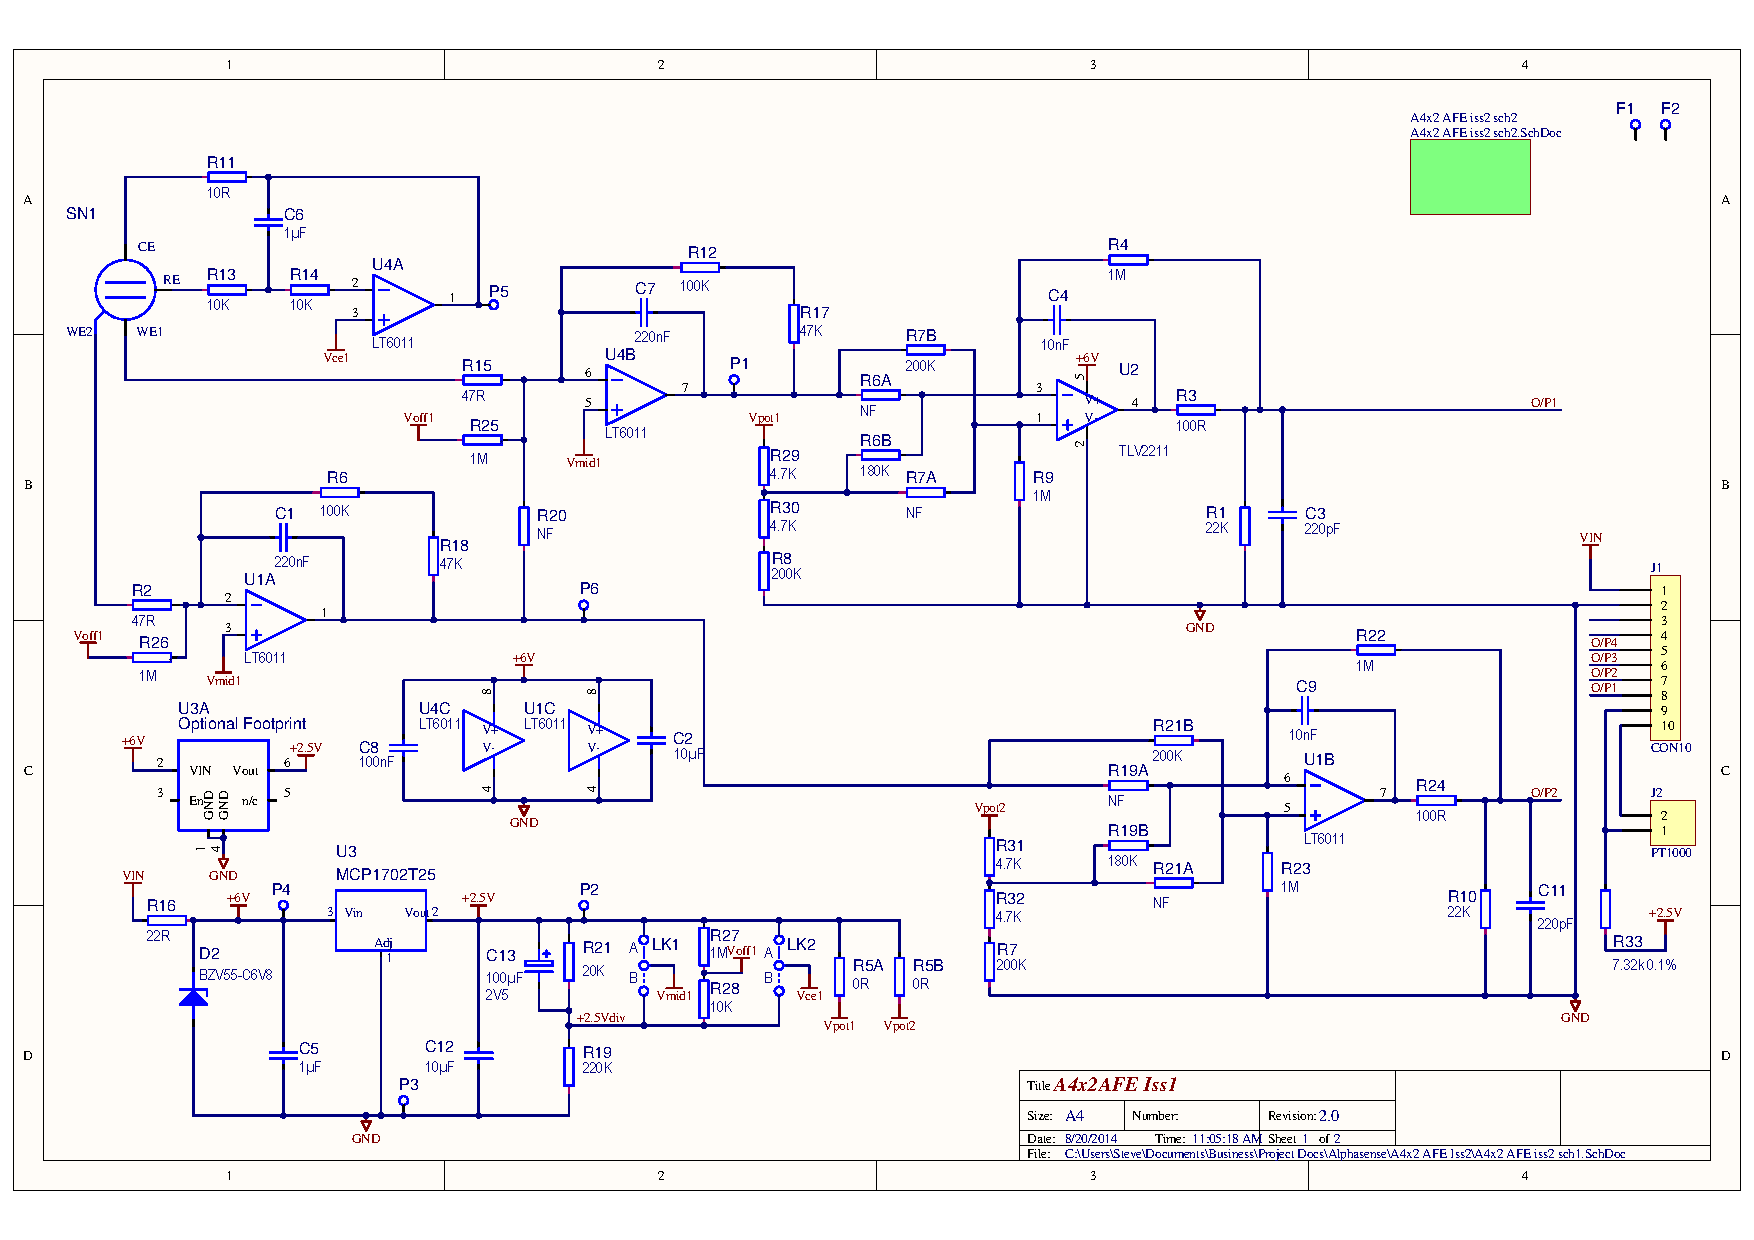
\includegraphics[page=1,width=.45\textwidth]{Pics/5.pdf}
%		\end{tabular}
%		\caption{Test}
%		\label{fig:Test}
%	\end{figure}
	


\begin{figure}
	\begin{center}
		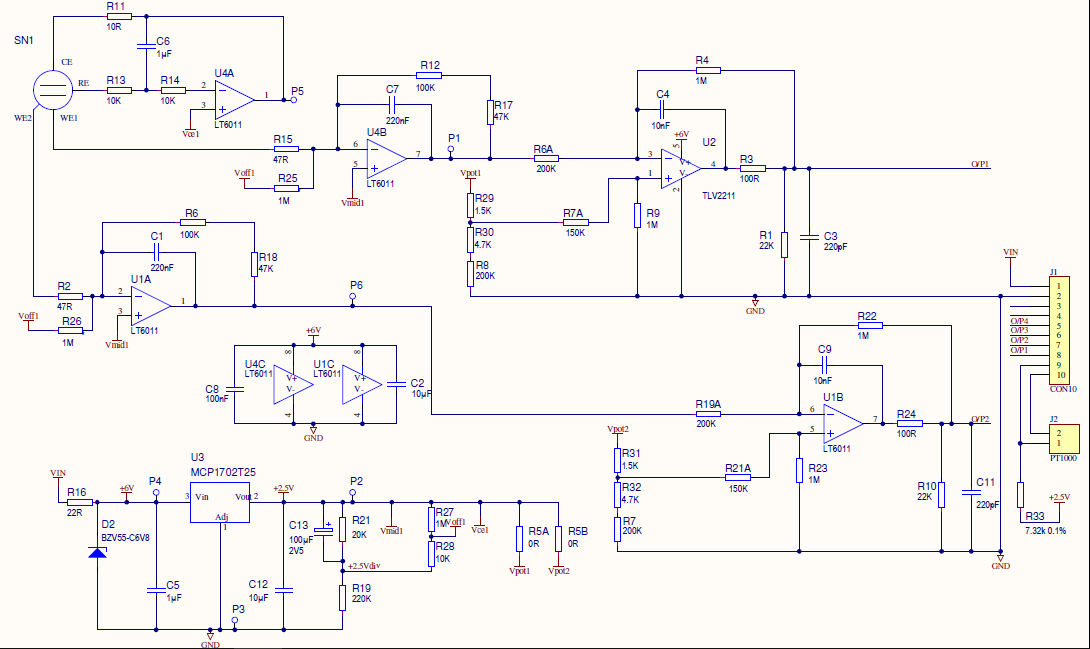
\includegraphics[width=1\textwidth]{Pics/6}
		\caption{Last Circuit Schematic}
		\label{fig:A.3}
		\vspace{1.2cm}
		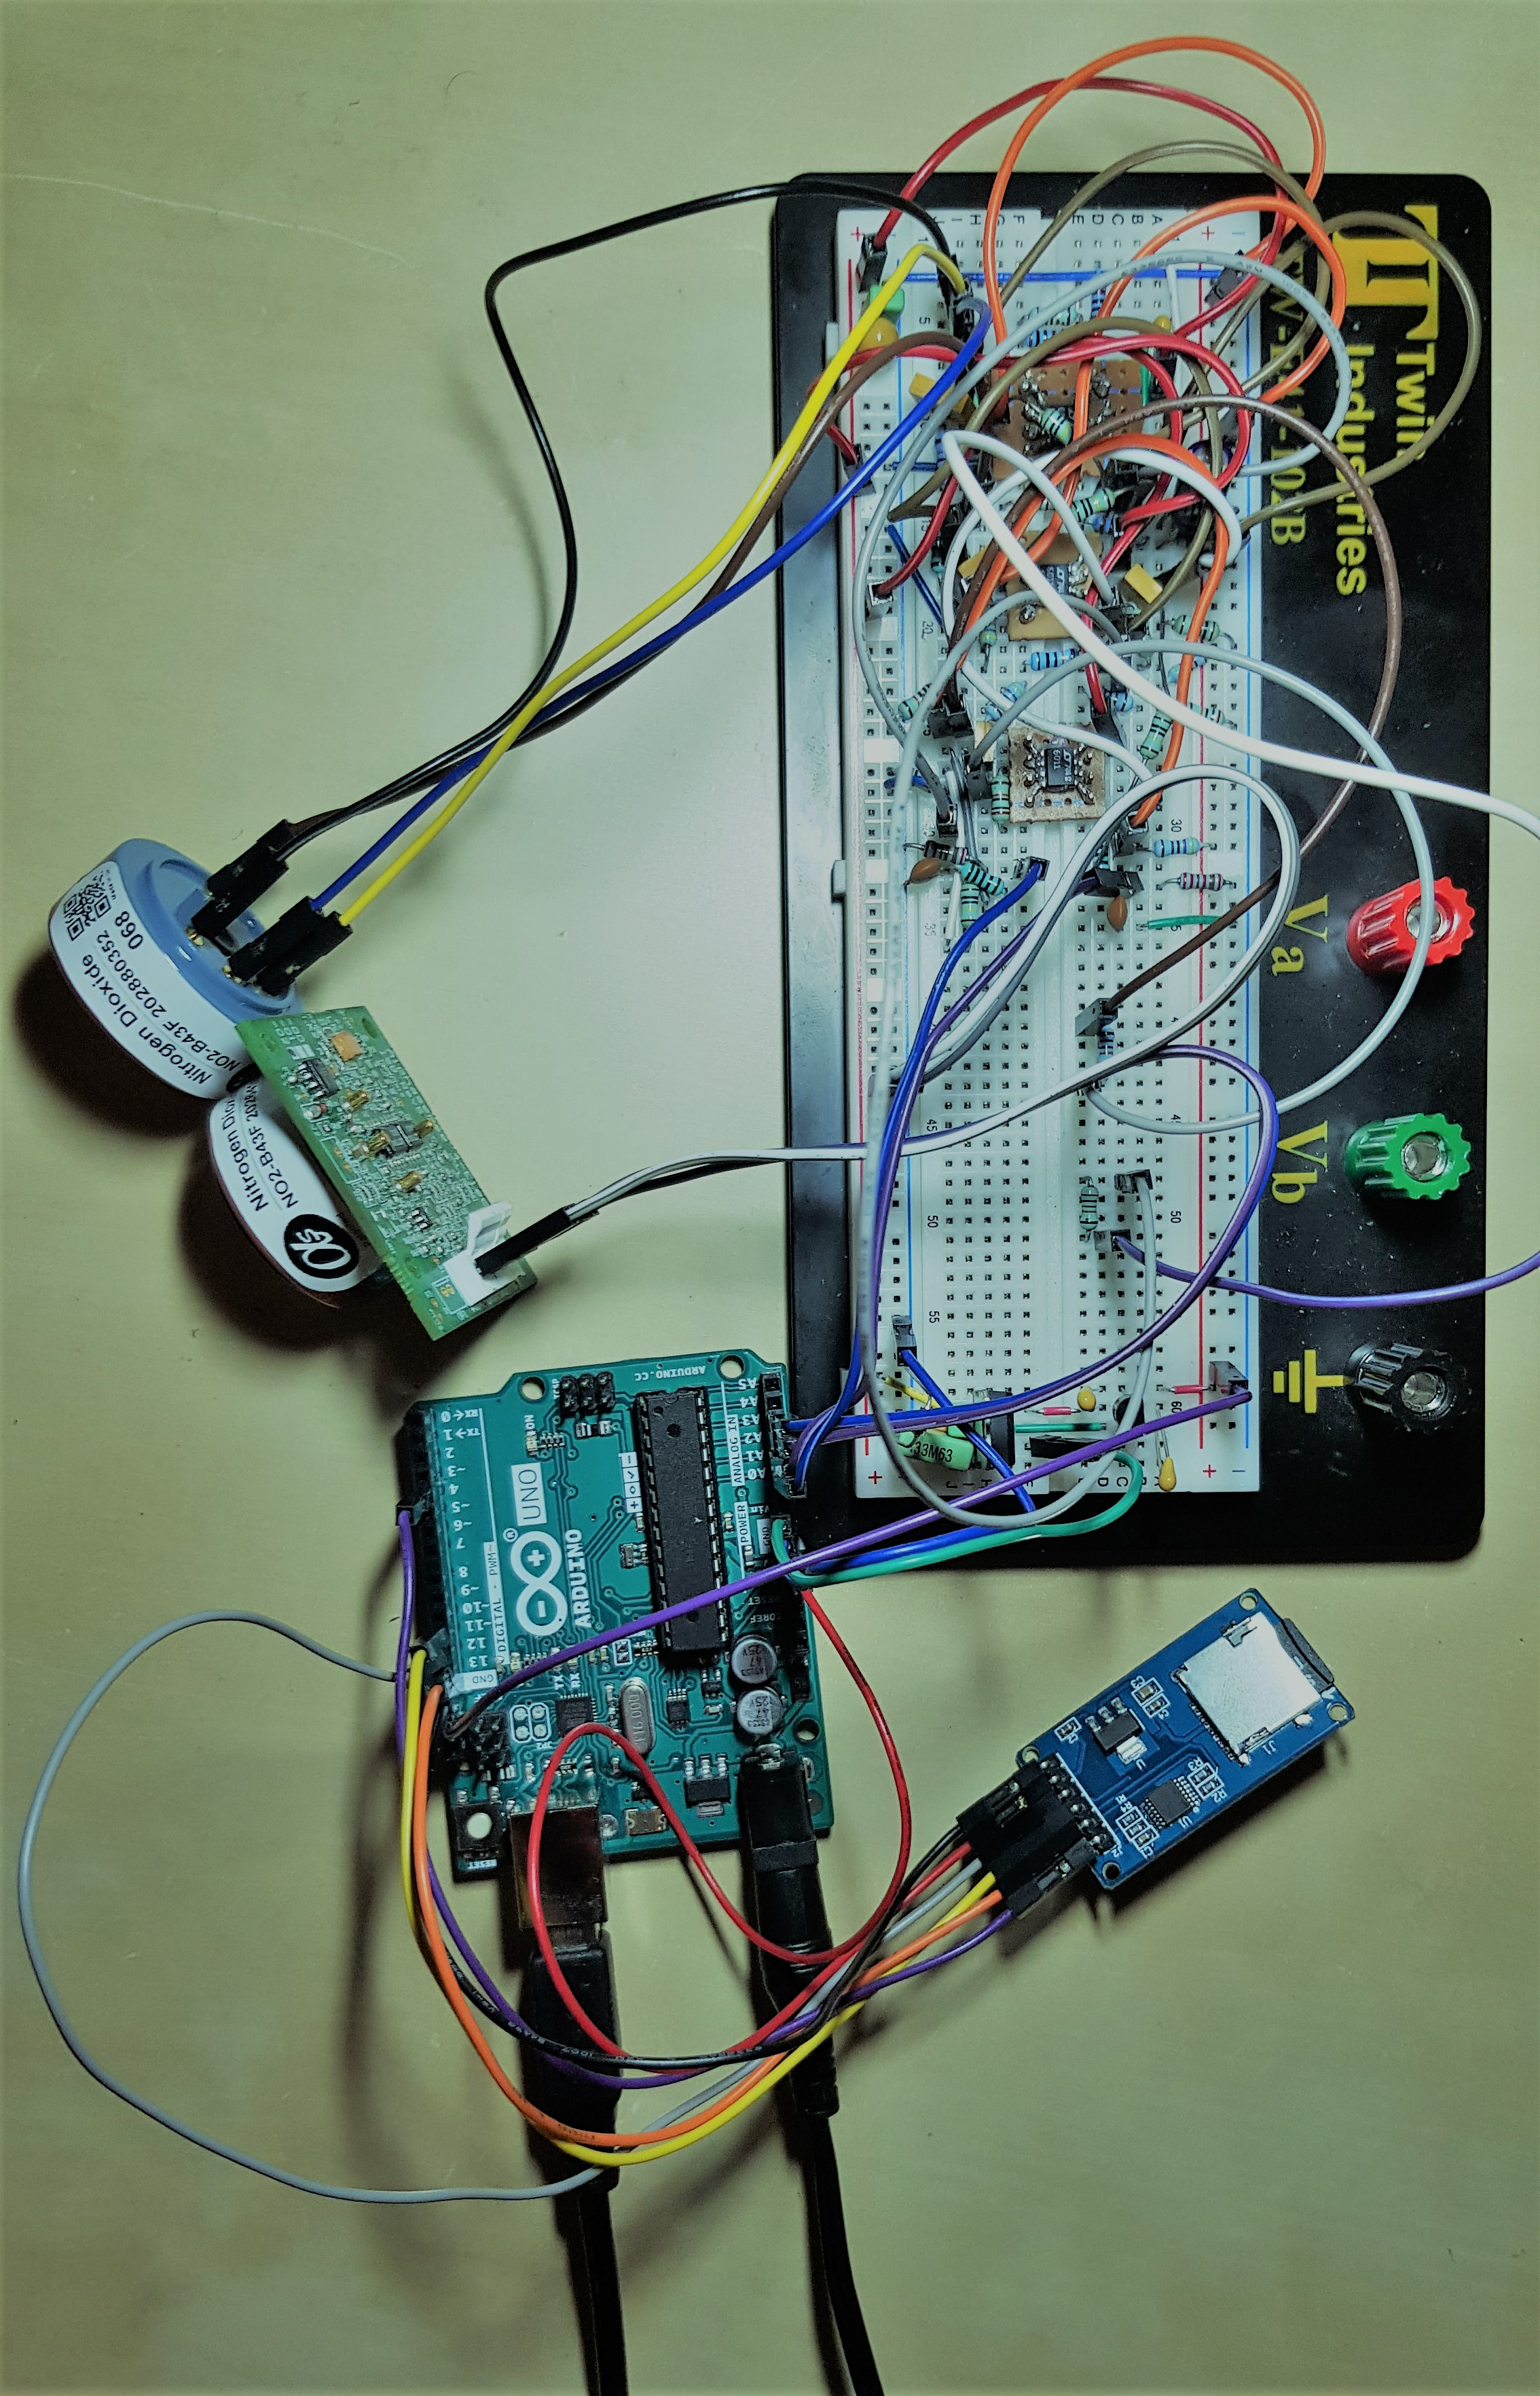
\includegraphics[width=0.5\textwidth]{Pics/7}
		\caption{Realization of the Circuit}
		\label{fig:A.4}
		\medskip
		%\small
		%Explanation
	\end{center}
\end{figure}

\chapter{Source Code}
\label{sub:appendixA}

\begin{lstlisting}[caption=Arduino Code,label=code:label]
#include <TimeLib.h>
#include <SPI.h>
#include <SD.h>

#define TIME_HEADER  "T"   // Header tag for serial time sync message
#define TIME_REQUEST  7    // ASCII bell character requests a time sync message 

const int chipSelect = 4;

void setup()  {
Serial.begin(9600);
analogReference(EXTERNAL);
//while (!Serial) ; // Needed for Leonardo only
pinMode(5, OUTPUT);

setSyncProvider( requestSync);  //set function to call when sync required
Serial.println("Waiting for sync message");

Serial.print("Initializing SD card...");

// see if the card is present and can be initialized:
if (!SD.begin(chipSelect)) {
Serial.println("Card failed, or not present");
// don't do anything more:
while (1);
}
Serial.println("Card Initialized");

}

void loop() {

if (Serial.available()) {
processSyncMessage();
}
if (timeStatus() == timeSet) {
digitalWrite(5, HIGH); // LED on if synced
} else {
digitalWrite(5, LOW);  // LED off if needs refresh
}

String dataString = "";

dataString += String(analogRead(A0)) + " & "  + String(analogRead(A1)) + " & " + String(analogRead(A2)) + " & "  + String(analogRead(A3)) + "  @  " + String(hour()) + ":" + String(minute()) + ":" + String(second()) + " ; " + String(day()) + "/" + String(month()) + "/" + String(year());

File dataFile = SD.open("datalog.txt", FILE_WRITE);

// if the file is available, write to it:
if (dataFile) {
dataFile.println(dataString);
dataFile.close();
// print to the serial port too:
Serial.println(dataString);
}
// if the file isn't open, pop up an error:
else {
Serial.println("error opening datalog.txt");
}

delay(1000);
}

void processSyncMessage() {
unsigned long pctime;
const unsigned long DEFAULT_TIME = 1357041600; // Jan 1 2013

if (Serial.find(TIME_HEADER)) {
pctime = Serial.parseInt();
if ( pctime >= DEFAULT_TIME) { // check the integer is a valid time (greater than Jan 1 2013)
setTime(pctime); // Sync Arduino clock to the time received on the serial port
}
}
}

time_t requestSync()
{
Serial.write(TIME_REQUEST);
return 0; // the time will be sent later in response to serial mesg
}

\end{lstlisting}

